\documentclass[11pt]{scrartcl}
\usepackage{ucs}
\usepackage[utf8x]{inputenc}
\usepackage{ngerman}
\usepackage{amsmath,amssymb,amstext}
\usepackage{amsthm}
\usepackage{graphicx}
\usepackage[automark]{scrlayer-scrpage}
\usepackage{hyperref}
\usepackage{listings}
\usepackage{cancel}

\pagestyle{scrheadings}

\title{Inverse shortest paths in directed acyclic graphs}
\author{Sven O. Krumke, Florian Dahms, Orges Leka (o.leka@th-bingen.de)}
\date{\today{} in Limburg}

\newtheorem{proposition}{Proposition}[section]
\newtheorem{lemma}[proposition]{Lemma}
\newtheorem{remark}[proposition]{Bemerkung}
\newtheorem{definition}{Definition}[section]


\begin{document}

\maketitle

\tableofcontents

\section{Inverse shortest paths}
\label{sec:ikw}

In the article 'Burton and Toint - 1992 - On an instance of the inverse shortest paths problem.', the following problem is solved: Edge costs in a directe graph are already given, and shortest paths are also provided. The objective is to find additional edge costs that explain the shortest paths and additionally minimize the $l_2$ norm with respect to the given costs. The problem is formulated as a quadratic optimization problem and solved using a polynomial-time method in $n$ steps, where $n$ is the number of nodes. 

The idea in the following proposition is to solve a related problem by considering a directed acyclic graphs with a topological sorting and to perform this sorting on a line that can represent a shortest path in the plane. Every path with nodes on this line is then a shortest path if we consider the distances on the line between the nodes as the new weighting. Since there can be different lines that satisfy this property, we later aim to select a line that attempts to minimize the sum of the distances from the original positions of the nodes in the plane to their respective positions on the line as much as possible.
\begin{center}
  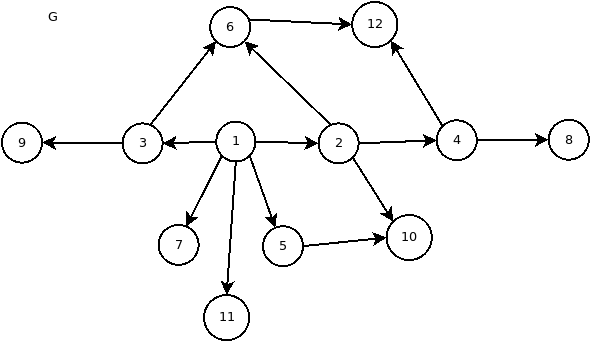
\includegraphics[width=0.7\textwidth]{Figur01.png}
\end{center}

\begin{center}
  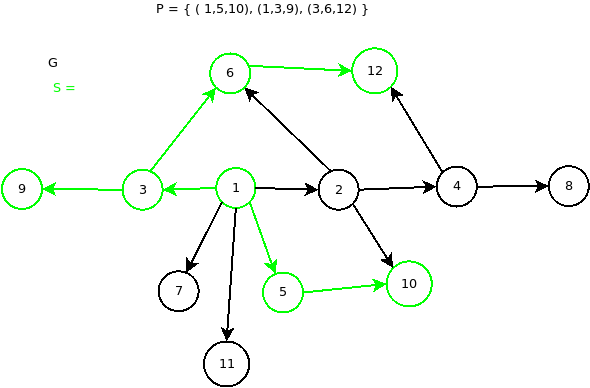
\includegraphics[width=0.7\textwidth]{Figur02.png}
\end{center}

\begin{center}
  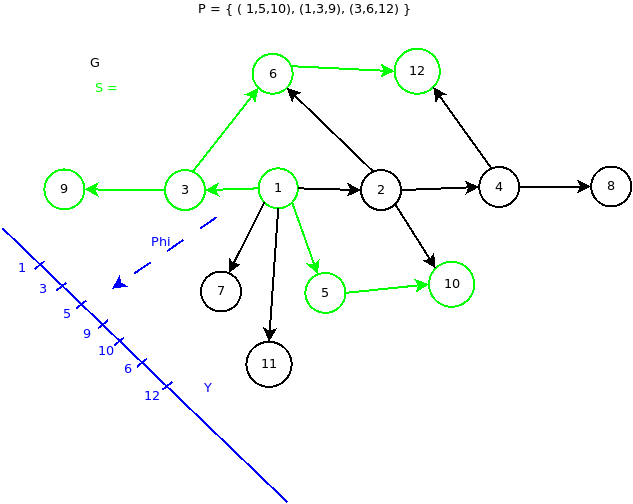
\includegraphics[width=0.7\textwidth]{Figur03.png}
\end{center}

\begin{proposition}
Let there be a directed acyclic graph $G = (V,E)$, where $\phi: V \rightarrow \mathbb{R}^2$ represents the position function, and $c(u,v) := |\phi(u)-\phi(v)|$ serves as the cost function on the edges. Additionally, we have a set of paths $P = \{p_1,\cdots,p_r\}$, and let $S = \left < P \right >_G$ be the graph $S=(V_S,E_S)$ generated by $P$ within $G$. Furthermore, consider an arbitrary line $Y = \{ y \in \mathbb{R}^2| y = x_0 + t r , \left < x_0, r \right > = 0, \left < r,r\right > = 1 , t \in \mathbb{R}\}$ defined by a point $x_0 \in \mathbb{R}^2$ on the line and a normalized direction vector $r \in \mathbb{R}^2$ of the line. We assume the existence of an injective mapping $\psi:V \rightarrow Y$.

Let $V = \{v_1,\cdots,v_n\}$ and $v_1 \trianglelefteq v_2 \trianglelefteq \cdots \trianglelefteq v_n$ represent a topological ordering of the nodes in $G$. For $u,v \in V$, define $u \le v :\iff \left < \psi(u), r \right > \le \left <\psi(v), r \right >$. We assume that $v_i \leq v_j \iff v_i \trianglelefteq v_j$, meaning that, according to this assumption, $v_1 \le v_2 \le \cdots \le v_n$ holds due to the topological ordering.

Let $m:= \min_{ (u,v) \in E, u \notin V_S \text{ or } v \notin V_S} |\phi(u)-\phi(v)|$ and $R:=|\psi(v_1)-\psi(v_n)|$. Define $\hat{c}(u,v)$ as:

\[
\hat{c}(u,v) = 
\begin{cases}
|\phi(u)-\phi(v)|, & \text{if } u \notin V_S \text{ or } v \notin V_S, \\
|\psi(u)-\psi(v)|\cdot \frac{m}{R}, & \text{if } u \in V_S \text{ and } v \in V_S.
\end{cases}
\]

Each path $p = (p_1,\cdots,p_k) \in P$ is then a shortest path under $\hat{c}$.

\end{proposition}
\begin{proof}
First, we observe that for $u, v \in V$, it holds:

\[
|\psi(u)-\psi(v)| = | \left < \psi(u), r\right > - \left < \psi(v), r\right >|
\]

This is because: Since $\psi(u)$ and $\psi(v)$ lie on the line $Y$, there exist $t_u$ and $t_v \in \mathbb{R}$ such that:

\[
\psi(u) = x_0 + t_u r, \quad \psi(v) = x_0 + t_v r
\]

From this, considering $|r| = 1$, we have:

\[
|\psi(u)-\psi(v)| = |t_u-t_v|
\]

On the other hand, we have:

\[
| \left < \psi(u), r\right > - \left < \psi(v), r\right >| = | \left < x_0 + t_u r, r\right > - \left < x_0 + t_v r, r\right >|
\]

And since $\left < x_0,r \right>=0$ and $\left < r,r\right> = 1$, it follows:

\[
= |t_u-t_v| = |\psi(u)-\psi(v)|
\]

We also notice that for $x, y, z \in V$ with $x \le y \le z$, it holds:

\[
|\psi(x)-\psi(z)| = |\psi(x)-\psi(y)| + |\psi(y)-\psi(z)|
\]

This holds because there exist $t_x, t_y, t_z \in \mathbb{R}$ such that $\psi(x) = x_0 + t_x r$, $\psi(y) = x_0 + t_y r$, and $\psi(z) = x_0 + t_z r$. Due to $x \le y \le z$, we have $t_x = \left < \psi(x) , r\right > \le t_y = \left < \psi(y) , r \right> \le t_z = \left < \psi(z), r \right >$, and it follows:

\[
|\psi(x)-\psi(z)| = |t_z-t_x| = t_z - t_x = t_z -t_y+t_y-t_x = |t_z-t_y| + |t_y-t_x| = |\psi(z)-\psi(y)| + |\psi(y)-\psi(x)|
\]

We also observe that for all $(u,v) \in E$, it holds:

\[
R = |\psi(v_1)-\psi(v_n)| \ge | \psi(u)-\psi(v)|
\]

This is because according to the assumption:

$v_1 \trianglelefteq u \trianglelefteq v \trianglelefteq v_n$

Which means:

$v_1 \le u \le v \le v_n$

Thus, based on the previous observation, it also holds that:

$R = |\psi(v_1)-\psi(v_n)| = |\psi(v_1)-\psi(u)| + |\psi(u)-\psi(v)|+|\psi(v)-\psi(v_n)| \ge |\psi(u)-\psi(v)|$

According to the definition of $\hat{c}$, for all $(u,v) \in E$, $u \in V_S$ and $v \in V_S$, it holds:

\[
\hat{c}(u,v) = |\psi(u)-\psi(v)| \cdot \frac{m}{R} \le 1 \cdot m = m
\]

According to the definition of $m$ and $\hat{c}$, for all $(u,v) \in E$, $u \notin V_S$ or $v \notin V_S$, it holds:

\[
\hat{c}(u,v) = |\phi(u)-\phi(v)| \ge m
\]

Now, let $p = (p_1,\cdots,p_k) \in P$ be a path from $P$. Let $q = (q_1,\cdots,q_l)$ be a path in $G$ with $q_1 = p_1$, $q_l = p_k$. We need to show that:

\[
\hat{c}(p) := \sum_{i=1}^{k-1} \hat{c}(p_i,p_{i+1}) \le^{\text{to be shown}} \sum_{i=1}^{l-1} \hat{c}(q_i,q_{i+1}) =:\hat{c}(q)
\]

Since $p \in P$ is a path in $G$, and $S = \left < P \right >_G$ as a subgraph of a directed acyclic graph is also directed and acyclic, it follows that:

$p_1 \trianglelefteq p_2 \trianglelefteq \cdots \trianglelefteq p_k$

where $\trianglelefteq$ is the topological ordering as defined above. According to the assumption on $\psi$, it holds:

$p_1 \le p_2 \le \cdots \le p_k$

Using the $\Delta$-inequality, we have:

\[
|\psi(p_1) -\psi(p_k)| \cdot \frac{m}{R} \le^{\Delta\text{-Ineq.}} \sum_{i=1}^{k-1} | \psi(p_i)-\psi(p_{i+1})| \cdot \frac{m}{R} = \sum_{i=1}^{k-1} \hat{c}(p_i,p_{i+1}) = \hat{c}(p)
\]

Furthermore, using the $\Delta$-inequality again, because the $\psi(p_j)$ are sorted by $\le$ on the line $Y$ (as per the assumption $v_i \leq v_j \iff v_i \trianglelefteq v_j$ for $\psi$), we have:

\[
\sum_{i=1}^{k-1} | \psi(p_i)-\psi(p_{i+1})| \cdot \frac{m}{R} =|\psi(p_1) -\psi(p_k)| \cdot \frac{m}{R}
\]

It follows:

\[
\hat{c}(p)=|\psi(p_1) -\psi(p_k)| \cdot \frac{m}{R}
\]

If now $q$ is a path whose nodes are all in $S$, the same argument shows that:

\[
\hat{c}(q) = |\psi(q_1) -\psi(q_l)| \cdot \frac{m}{R} = |\psi(p_1)-\psi(p_k)| \cdot \frac{m}{R} = \hat{c}(p)
\]

Otherwise, there exists a $j$ such that $q_j$ is not in $V_S$. We denote by $I$ the set of indices $i$ such that $q_i \in V_S$ and $q_{i+1} \in V_S$, and by $I^c$ the set of indices $i$ with $q_i \notin V_S$ or $q_{i+1} \notin V_S$, i.e.:

$I := \{i| 1 \le i \le l-1, q_i \in V_S \text{ and } q_{i+1} \in V_S\}$

and

$I^c := \{i| 1 \le i \le l-1, q_i \notin V_S \text{ or } q_{i+1} \notin V_S\}$

We then have:

\[
\hat{c}(q) = \sum_{1 \le i \le l-1} \hat{c}(q_i,q_{i+1}) = \sum_{i \in I} \hat{c}(q_i,q_{i+1})+\sum_{i \in I^c} \hat{c}(q_i,q_{i+1})=\ldots
\]

However, for $i \in I$, it holds:

\[
\hat{c}(q_i,q_{i+1}) = |\psi(q_i)-\psi(q_{i+1})| \cdot \frac{m}{R}
\]

And for $i \in I^c$, it holds:

\[
\hat{c}(q_i,q_{i+1}) \ge m = 1 \cdot m \ge |\psi(q_i)-\psi(q_{i+1})| \cdot \frac{m}{R}
\]

It follows:

\[
\ldots=\sum_{i \in I} \hat{c}(q_i,q_{i+1})+\sum_{i \in I^c} \hat{c}(q_i,q_{i+1}) \ge \frac{m}{R} \sum_{1 \le i \le l-1}{|\psi(q_i)-\psi(q_{i+1})|}
\]

\[
=\frac{m}{R} |\psi(q_1)-\psi(q_l)|=\frac{m}{R} |\psi(p_1)-\psi(p_k)| = \hat{c}(p)
\]

Therefore, in this case, we have:

\[
\hat{c}(q) \ge \hat{c}(p)
\]

Overall, it follows that $p$ is a shortest path under $\hat{c}$.
\end{proof}

\hrulefill

Given:
- $\mathbf{c}(u,v):=$ Currently used costs
- $\hat{c}(u,v):=$ Shortest path costs
   (Here, $\hat{c}(u,v):=$ costs that exactly represent the shortest paths on the given paths)

Approach (from Johnson's or Surballee's Algorithm):
Desired: Potential function $h: V \rightarrow \mathbb{R}$ that minimizes $(*):$

$$ (*): \min_{h} \sum_{(u,v) \in E} (\mathbf{c}(u,v)-(\hat{c}(u,v)+h_v-h_u))^2 \text{ and } \gamma(u,v):= \hat{c}(u,v) + h_v-h_u\ge^! 0$$

Heuristic solution approach:
Let $s \in V$. Define: $\hat{h}_s(v) = d_{\mathbf{c}}(s,v) = $ distance of the shortest path with $\mathbf{c}$ from $s$ to $v$ (Here, $s$ is a source: $\forall v \in V \exists$ a path from $s$ to $v$. If there is no such $s$, we sort the directed acyclic graph $G$ using topological sorting and add a new node $s$ by connecting this node $s$ with all nodes $x$ having an in-degree $\deg^-(x)=0$ and setting the cost of this connection to $\mathbf{c}(s,x):=0$. Then, $s$ has the desired property that there is a path from $s$ to every $v \in V$.) ($\hat{h}_s(v)$ is calculated as in the Johnson's algorithm using the Bellman-Ford algorithm: Runtime $(|E||V|)$).
Then, it holds:

$$\mathbf{c}(u,v)+\hat{h}_s(v)-\hat{h}_s(u) \ge d_{\mathbf{c}}(u,v) + \hat{h}_s(v)-\hat{h}_s(u) = d_{\mathbf{c}}(u,v)+d_{\mathbf{c}}(s,v)-d_{\mathbf{c}}(s,u) \ge^{\Delta-\text{Ineq.}} 0$$

We calculate using isometric regression:

$$\min_{h} \sum_{i=1}^n(\hat{h}_s(v_i)-h_{v_i})^2$$

subject to the constraint $h_u \le h_v \forall (u,v) \in E$ (Runtime $O(|V|)$).
We then set $\gamma(u,v):=\underbrace{\hat{c}(u,v)}_{\ge 0} + \underbrace{h_v-h_u}_{\ge 0} \ge 0$.

The potential function $h_v$ generally does not minimize equation $(*)$.

By using a potential function $h_v$ and transforming the weights $\hat{c}(u,v)$ to $\gamma(u,v) = \hat{c}(u,v)+h_v-h_u$, we maintain the property of shortest paths. 

Proof: 

Let $p$ be a shortest path under $\hat{c}$ from $p_1$ to $p_k$. Then, for all paths $q$ from $q_1 = p_1$ to $q_l = p_k$, it holds that:

$$\hat{c}(p) \le \hat{c}(q) $$

According to the definition of $\gamma(u,v):= \hat{c}(u,v) + h_v-h_u$, we have:

$$\gamma(p) := \sum_{i=1}^{k-1} \gamma(p_i,p_{i+1}) = \sum_{i=1}^{k-1} \hat{c}(p_i,p_{i+1})+h_{p_{i+1}}-h_{p_{i}} $$

$$=^\text{ Telescoping sum } (\sum_{i=1}^{k-1} \hat{c}(p_i,p_{i+1}))+(h_{p_k}-h_{p_1})$$
$$ = \hat{c}(p)+h_{p_k}-h_{p_1} \le \hat{c}(q)+h_{q_l}-h_{q_1} = \gamma(q)$$

Thus, $\gamma(p) \le \gamma(q)$, and $p$ is also a shortest path under $\gamma$.
\end{document}



